\documentclass[tikz, border=1mm]{standalone}
\usepackage{tikz} 
\usetikzlibrary{arrows.meta}
\usepackage{pgfplots}

\begin{document}

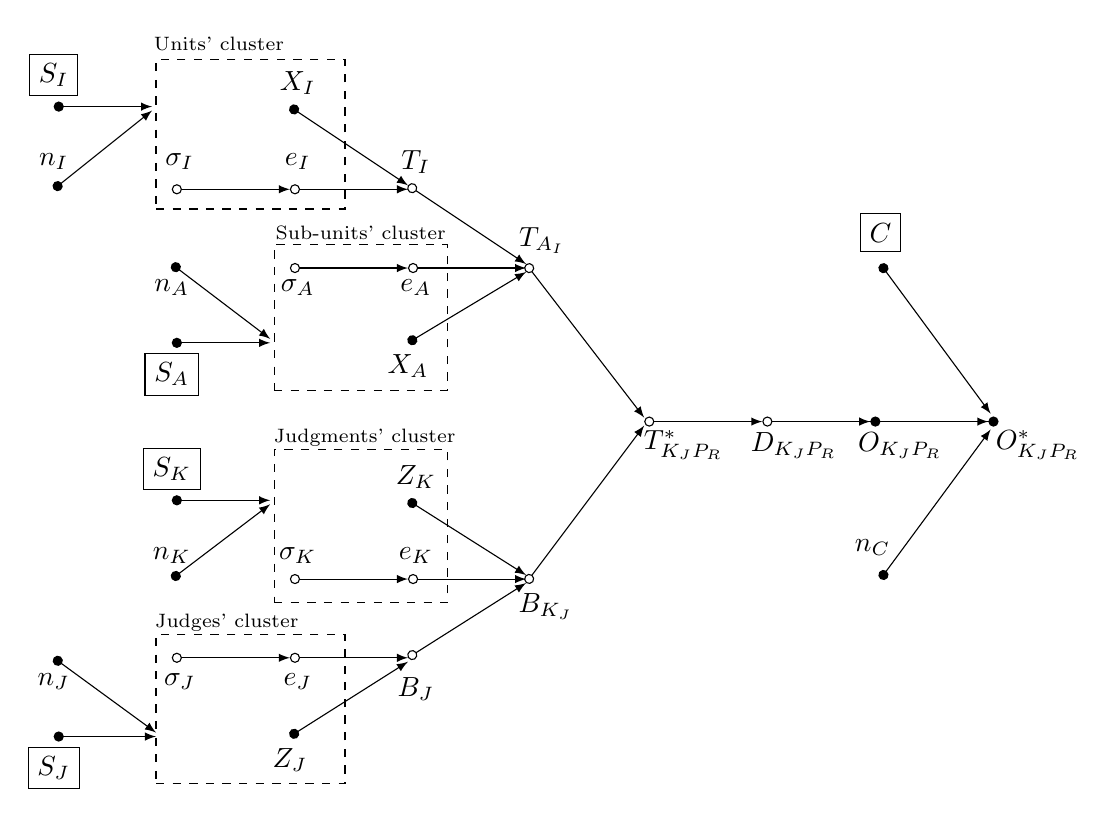
\begin{tikzpicture}

    % complete outcome
    \node at (3.25,0.7) {$O_{{K_{J}P_{R}}}$}; %[gray]
    
    % discriminal difference
    \node at (1.9,0.7) {$D_{{K_{J}P_{R}}}$}; %[gray]
    \draw[{Circle[open]}-{latex}{Circle}](1.5,1) to (3,1); %,gray
    
    % "perceived" discriminal process for vector of stimulus
    \node at (0.5,0.7) {$T^{*}_{K_{J}P_{R}}$}; %[gray]
    \draw[{Circle[open]}-{latex}](0,1) to (1.5,1); %,gray

    % "true" discriminal process for sub-unit
    \node at (-1.3,3.3) {$T_{A_{I}}$}; %[gray]
    \draw[{Circle[open]}-{latex}](-1.5,3) to (0,1.05); %,gray

    % repeated judges' bias k_{j}
    \node at (-1.25,-1.35) {$B_{K_{J}}$}; %[gray]
    \draw[{Circle[open]}-{latex}](-1.5,-1.05) to (0,0.95); %,gray

    % "true" discriminal process of unit
    \node at (-2.9,4.3) {$T_{I}$}; %[gray]
    \draw[{Circle[open]}-{latex}](-3,4) to (-1.5,3); %,gray

    % sub-units error
    \node at (-2.9,2.7) {$e_{A}$}; %[gray]
    \draw[{Circle[open]}-{latex}](-3,2.95) to (-1.5,2.95); %,gray
    
    % predictors for sub-unit
    \node at (-3,1.7) {$X_{A}$}; %[gray]
    \draw[{Circle}-{latex}](-3,2) to (-1.5,2.90); %,gray

    % sub-units population size
    \node at (-4.4,2.7) {$\sigma_{A}$}; %[gray]
    %\draw[{Circle}-{latex}](-4.5,2.95) to (-3,2.95); %,gray
    \draw[{Circle[open]}-{latex}](-4.5,2.95) to (-3,2.95); %,gray

    % square around sub(units)
    \node[font=\scriptsize] at (-3.6,3.4) {Sub-units' cluster}; %,gray
    \draw[dashed] (-4.7,1.4)--(-2.5,1.4)--(-2.5,3.25)--(-4.7,3.25)--(-4.7,1.4); %,gray

    % predictors for units
    \node at (-4.4,5.3) {$X_{I}$}; %[gray]
    \draw[{Circle}-{latex}](-4.5,5) to (-3,4); %,gray

    % units trait error
    \node at (-4.4,4.3) {$e_{I}$}; %[gray]
    \draw[{Circle[open]}-{latex}](-4.5,3.95) to (-3,3.95); %,gray

    % units population size
    \node at (-5.9,4.3) {$\sigma_{I}$}; %[gray]
    %\draw[{Circle}-{latex}](-6,3.95) to (-4.5,3.95); %,gray
    \draw[{Circle[open]}-{latex}](-6,3.95) to (-4.5,3.95); %,gray

    % square around sub(units)
    \node[font=\scriptsize] at (-5.4,5.8) {Units' cluster}; %[gray]
    \draw[dashed] (-6.2,3.7)--(-3.8,3.7)--(-3.8,5.6)--(-6.2,5.6)--(-6.2,3.7); %,gray

    % judgments' bias error
    \node at (-2.9,0.3) {$Z_{K}$}; %[gray]
    \draw[{Circle}-{latex}](-3,0) to (-1.5,-0.95); %,gray
    
    % predictors for repeated judges' bias
    \node at (-2.9,-0.7) {$e_{K}$}; %[gray]
    \draw[{Circle[open]}-{latex}](-3,-1) to (-1.5,-1); %,gray

    % repeated comparisons population size
    \node at (-4.4,-0.7) {$\sigma_{K}$}; %[gray]
    %\draw[{Circle}-{latex}](-4.5,-1) to (-3,-1); %,gray
    \draw[{Circle[open]}-{latex}](-4.5,-1) to (-3,-1); %,gray

    % judges' bias
    \node at (-2.9,-2.4) {$B_{J}$}; %[gray]
    \draw[{Circle[open]}-{latex}](-3,-2) to (-1.5,-1.05); %,gray

    % square around sub(units)
    \node[font=\scriptsize] at (-3.55,0.8) {Judgments' cluster}; %[gray]
    \draw[dashed] (-4.7,-1.3)--(-2.5,-1.3)--(-2.5,0.65)--(-4.7,0.65)--(-4.7,-1.3); %,gray

    % predictors for judges' bias
    \node at (-4.5,-3.3) {$Z_{J}$}; %[gray]
    \draw[{Circle}-{latex}](-4.5,-3) to (-3,-2.05); %,gray

    % judges' bias error
    \node at (-4.4,-2.3) {$e_{J}$}; %[gray]
    \draw[{Circle[open]}-{latex}](-4.5,-2) to (-3,-2); %,gray

    % judges' population size
    \node at (-5.9,-2.3) {$\sigma_{J}$}; %[gray]
    %\draw[{Circle}-{latex}](-6,-2) to (-4.5,-2);
    \draw[{Circle[open]}-{latex}](-6,-2) to (-4.5,-2); %,gray

    % square around sub(units)
    \node[font=\scriptsize] at (-5.30,-1.55) {Judges' cluster}; %[gray]
    \draw[dashed] (-6.2,-3.6)--(-3.8,-3.6)--(-3.8,-1.7)--(-6.2,-1.7)--(-6.2,-3.6); %,gray

    %%%%%%%%%%%%%%%%%%%%%%%%%%%%%%%%%%%%%%%%%%%%%%%%%%%%%%
    
    % sampling mechanism (units)
    \node[rectangle,draw] at (-7.5,5.4) {$S_{I}$}; %,gray
    \draw[{Circle}-{latex}](-7.5,5) to (-6.25,5); %,gray
    
    % units sample size
    \node at (-7.5,4.3) {$n_{I}$}; %[gray]
    \draw[{Circle}-{latex}](-7.5,3.95) to (-6.25,4.95); %,gray

    % sampling mechanism (subunits)
    \node[rectangle,draw] at (-6,1.6) {$S_{A}$}; %,gray
    \draw[{Circle}-{latex}](-6,3) to (-4.75,2.05); %,gray
    
    % subunits sample size
    \node at (-6,2.7) {$n_{A}$}; %[gray]
    \draw[{Circle}-{latex}](-6,2) to (-4.75,2); %,gray

    % sampling mechanism (repeated judgments)
    \node[rectangle,draw] at (-6,0.4) {$S_{K}$}; %,gray
    \draw[{Circle}-{latex}](-6,0) to (-4.75,0); %,gray
    
    % units sample size
    \node at (-6,-0.7) {$n_{K}$}; %[gray]
    \draw[{Circle}-{latex}](-6,-1) to (-4.75,-0.05); %,gray

    % sampling mechanism (judges)
    \node[rectangle,draw] at (-7.5,-3.4) {$S_{J}$}; %,gray
    \draw[{Circle}-{latex}](-7.5,-3) to (-6.2,-3); %,gray
    
    % judges sample size
    \node at (-7.5,-2.3) {$n_{J}$}; %[gray]
    \draw[{Circle}-{latex}](-7.5,-2) to (-6.2,-2.95); %,gray
    
    %%%%%%%%%%%%%%%%%%%%%%%%%%%%%%%%%%%%%%%%%%%%%%%%%%%%%%

    % comparison mechanism (selection mechanism)
    \node [rectangle,draw] at (3,3.4) {$C$}; %[gray]
    \draw[{Circle}-{latex}](3,3) to (4.4,1.1); %,gray
    
    % observed outcome
    \node at (5,0.7) {$O^{*}_{{K_{J}P_{R}}}$}; %[gray]
    \draw[-{latex}{Circle}](3,1) to (4.5,1); %,gray
    
    % comparison sample size
    \node at (2.9,-0.6) {$n_{C}$}; %[gray]
    \draw[{Circle}-{latex}](3,-1) to (4.4,0.9); %,gray
        
\end{tikzpicture}

\end{document}
